\section{HYPSO-1} \label{hypso-mission}
% \textcolor{blue}{Contribution (3): "We present the chosen spacecraft bus of HYPSO-1 and justify the feasibility of the concept based on the spacecraft capabilities in terms of its chosen subsystems as well as power, communications and data budget constraints."
% Key points to keep in mind while writing this section are:
% \begin{itemize}
%     \item How will the chosen HYPSO-1 bus (present an overview) enable the CONOPS discussed in section \ref{sec:mission-design}?
%     \item What are the key subsystems that impact the CONOPS discussed in section \ref{sec:mission-design}?
%      \item What are the constraints with using the HSI discussed in section \ref{sec:hsi} (and spacecraft constraints on HSI?)?
%     \item Justify with technical system budgets how the CONOPS is feasible as discussed in section \ref{sec:mission-design}
% \end{itemize}}
\subsection{Spacecraft Bus} \label{sec:spacecraft}
% The mission objectives drive the design of the system, and design decisions must be made at the operational, system, functional, logical and the physical levels. 
% \textcolor{red}{ to provide the capabilities required to satisfy the CONOPS discussed in section \ref{sec:mission-design}. However, the COTS-based design is subject to what is available, and trade-offs must be made in terms of performance and functionality for the system design. .}

% This section will describe the spacecraft and the subsystems selected to support the mission, and discuss the constraints and their impact on the system design and CONOPS.
\begin{figure}[htbp]
  \centering
      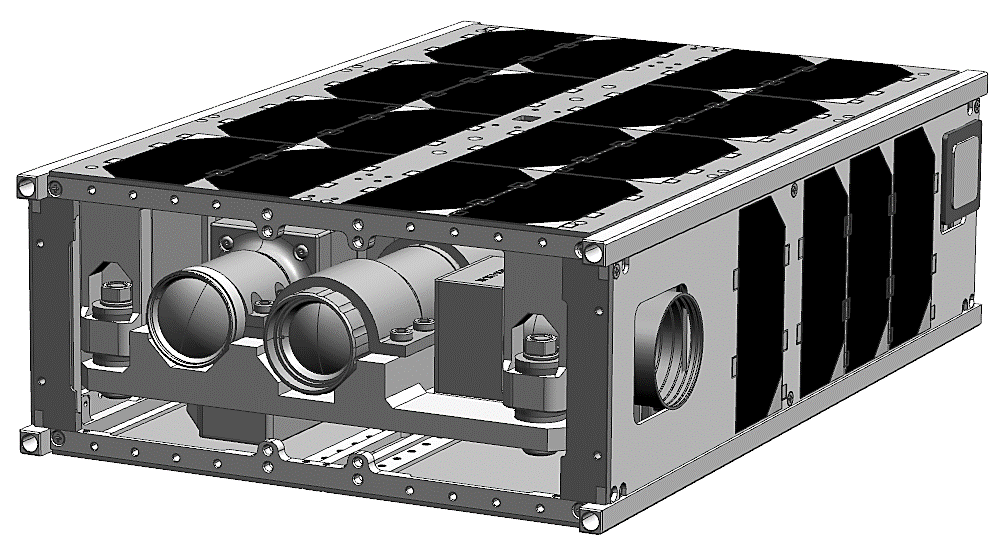
\includegraphics[width=0.4\textwidth]{figs/M6P.png}
  \caption{Isometric view of M6P with front panel removed showing the hyperspectral imager in the center, a RGB camera to its left and a star-tracker to its right.}
\end{figure}
Due to cost, schedule, and resources available, the hyperspectral imager, described in Section \ref{sec:hsi}, was chosen to be integrated to a commercially available spacecraft bus. The chosen bus is the Multipurpose 6U Platform (M6P) provided by NanoAvionics. The hyperspectral imager must adapt to existing bus interfaces which in turn affects the mission operations. Continuous iterations based on discussions with end users affected the mission and systems design concurrently, a common process in spacecraft development \cite{Ryschkewitsch2009,boehm1988,smad1999}. 
% The feasibility of CONOPS, described in section \ref{sec:mission-design}, can be determined by analysis of the power and data latency budgets.

Among the important subsystems of M6P are the Flight Computer (FC) for onboard data handling and ADCS functions, a SatLab Global Navigation Satellite System (GNSS) for accurate positioning and on-board time synchronization through a Pulse-per-Second (PPS) signal, Electrical Power System (EPS) for power management, a UHF Radio for basic communications, and a Payload Controller (PC) working as a network interface and router between the payload and the bus. All subsystems communicate over a CubeSat Space Protocol (CSP) and Controller Area Network (CAN) network, where each subsystem is a node with its own CSP address. To fulfill the CONOPS described in Section \ref{sec:mission-design}, the M6P is tailored to be equipped with: 
\begin{itemize}
    \item 16 triple junction solar cells made of Gallium Arsenide that charge six Lithium-Ion batteries with a combined energy capacity of approximately $64.9 \hspace{3pt} \rm{Wh}$, providing enough power for the planned sequences.
    \item A BICE NST-1B star-tracker with FoV of $21^{\circ}$ and measuring accuracy of $8 \hspace{3pt} \rm{arcsec}$ along the $x_b$ and $y_b$ axes and STIM 210 IMU with bias stability of $1.32\times 10^{-6}\rm{deg/s}$ and noise standard deviation of $8\times 10^{-3} \rm{deg/s}$, which are dedicated for the slew maneuver to provide precise attitude accuracy. To ensure sufficient settling time in the sensors' temperature-dependent bias and initialization in the attitude estimator algorithm, the sensors are turned on for at least $4 \hspace{3pt} \rm{min}$ prior imaging. Since the sensors consume a lot of power they are therefore scheduled to immediately turn off when the slew maneuver is complete. For operations without hyperspectral imaging, the M6P's six sun sensors, three magnetometers and three Micro-Electro-Mechanical-System (MEMS) gyroscopes are used instead when provide coarser attitude determination to relieve the power budget. 
    \item Four reaction wheels are used for attitude control and provide up to $3.2 \hspace{3pt} \rm{mNm}$ torque each, three being placed orthogonal to each other and the fourth at a $54.7^{\circ}$ angle with respect to the other three. 
    % Two magnetorquers, that may produce a maximum magnetic dipole of $0.46 \hspace{3pt} \rm{Am^2}$ each, are placed along each body axis and are used for reaction wheel momentum dumping.
    \item A RGB camera (IDS UI-125x, 6mm, f/1.4 Ci Series Fixed lens, with custom housing) that takes images with a footprint of $770 \hspace{3pt} \rm{km} \times 540 \hspace{3pt} \rm{km}$ and spatial resolution of approximately $500 \hspace{3pt} \rm{m}$, whose main purpose is to support and validate the orthorectification of hyperspectral images in the spatial domain \cite{habib2016ortho}.
    \item A $2.4 \hspace{3pt}  \rm{GHz}$ Satlab S-band Transceiver provides an usable data rate of up to $1 \hspace{3pt} \rm{Mbps}$ for downlink of payload data to the ground. 
    \item An Onboard Processing Unit (OPU) which is dedicated to fast image processing of hyperspectral data. It based on a Xilinx PicoZed SoC that consists of two core ARM processors and a Field Programmable Gate Array (FPGA). The FPGA enables reconfiguration of hardware for specific applications after launch. The PicoZed interfaces with the RGB and hyperspectral cameras through a customized breakoutboard. Large amounts of payload data need to be transferred from the OPU to the PC at a usable CAN speed of $0.4 \hspace{3pt} \rm{Mbps}$ before transmitting over the radio. It also hosts two SD-cards that allows storing up to $24 \hspace{3pt} \rm{GB}$ of data. 
\end{itemize}

\subsection{Power Budget}
Given that HYPSO-1 is in a $500 \hspace{3pt} \rm{km}$ SSO with Right Ascension of Ascending Node of $198.42^{\circ}$, the comprehensive results for the power budget are shown in Tables \ref{tab:power-budget}. The orbit is shown in Figure \ref{fig:orbit_hypso}.
\begin{figure}[tbhp]
  \begin{center}
    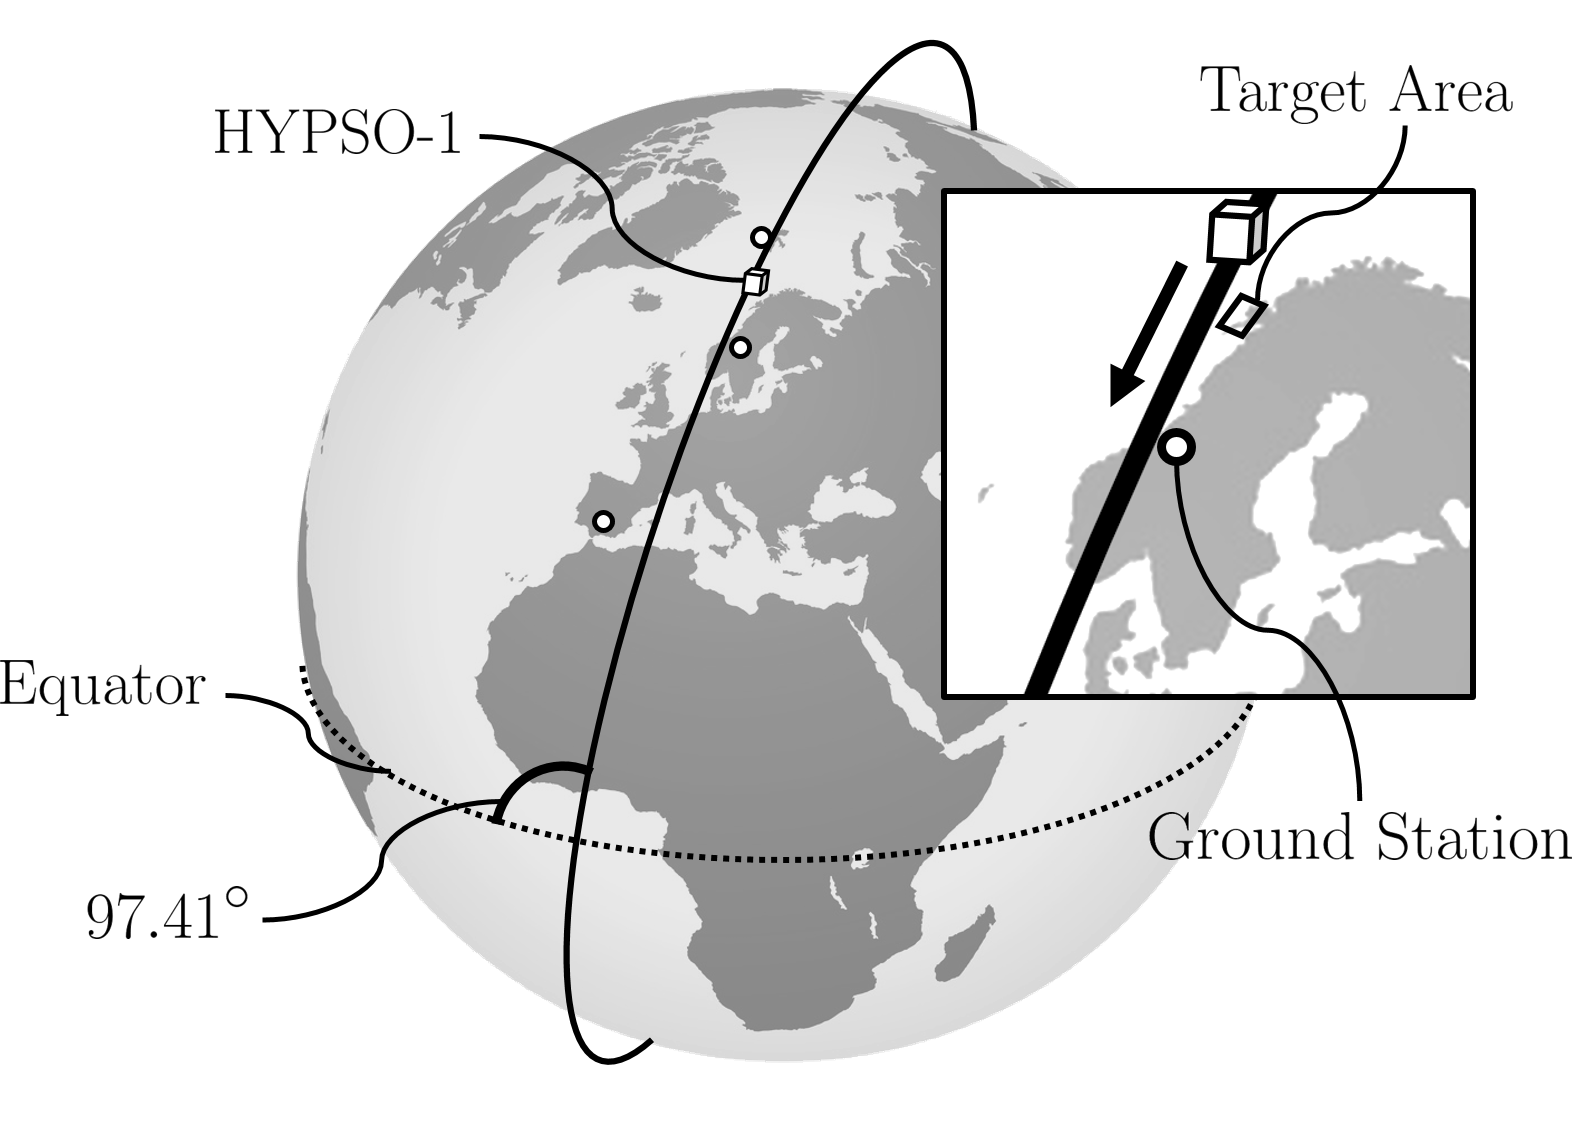
\includegraphics[width=85mm,angle=0]{figs/orbit_hypso.png}
    \caption{The orbit of HYPSO-1 at 10:11:17 on 15 August 2021. The target area is Lofoten, Norway. Selected ground stations at NTNU, KSAT Svalbard and KSAT Spain are represented by white circles.}
    \label{fig:orbit_hypso}
\end{center}
\end{figure}
\begin{table}[htbp]
	\caption{Power budget}
	\label{tab:power-budget}
	\centering
			\begin{tabular}{l r r r}
				\hline
				Battery Capacity & $64.90 \hspace{3pt} \rm{Wh}$ & & \\ 
				Generated Power & $11.65 \hspace{3pt} \rm{W}$ & & \\ 
			   Efficiency & $84.64 \hspace{3pt} \rm{\%}$ & & \\
			   \hline
			  Subsystem & Power ($\rm{W}$) & DC ($\%$) & Power Used ($\rm{W}$) \\
			  \hline
				Hyperspectral imager & 3.675 & 1.054 & 0.039 \\
				RGB camera & 3.360 & 0.019 & $6.384\times10^{-5}$ \\
				OPU imaging & 3.059 & 1.054 & 0.003 \\
			    OPU image processing & 2.315 & 4.76 & 0.146 \\
			    OPU CAN transfer & 2.132 & 35.33 & 0.753 \\
				ADCS normal & 4.765 & 94.77 & 4.516 \\
				ADCS precise & 7.907 & 5.23 & 0.414 \\
			    S-band radio RX & 4.813 & 10.57 & 0.509 \\
				S-band radio TX+RX & 12.201 & 10.57 & 1.290 \\
				Other & 1.153 & 100 & 1.153 \\
				\hline
				Total ($+10\%$ margin) &  & & 9.706 \\
				Remaining &  & & 0.155 \\
				\hline
				\end{tabular}
\end{table}

The M6P solar arrays are able to generate approximately $11.65 \hspace{3pt} \rm{W}$ during $3532 \hspace{3pt} \rm{s}$ out of the total orbit period of $5677 \hspace{3pt} \rm{s}$ (accounting for $2145 \hspace{3pt} \rm{s}$ time in eclipse). It is assumed that the input and output efficiencies of the batteries are $92 \%$ each. Table \ref{tab:power-budget} shows the physically measured nominal power ratings with $5 \%$ component margin and corresponding duty cycles (DC). The OPU, ADCS and S-band radio power ratings are distinguished into more than one operational mode, while "Other" denotes the collective power consumption by FC, EPS, PC and internal bus communications. In particular, high power consumption is expected during the HSI image acquisition and slew maneuver when the IMU and star-tracker are active, consuming up to $1.5 \hspace{3pt} \rm{W}$ each. Adding a $10 \%$ system margin results in remaining available power of about $0.155 \hspace{3pt} \rm{W}$. Constrained by the power budget, allowed downlink time is $10 \hspace{3pt} \rm{min}$ per orbit which means that potentially $75 \hspace{3pt} \rm{MB}$ of data may be downloaded. The allowed for transferring data through CAN is set to $33.42 \hspace{3pt} \rm{min}$ while the time for OPU on-board image processing can be set at a maximum of $270 \hspace{3pt} \rm{s}$.
% As the mission matures other parts of the processing pipeline can become a a part of the on-board processing and then the reconfigurability of the FPGA is a crucial feature to achieve the desired performance when dealing with gigabytes of hyperspectral data.
% \subsubsection{Communications}
% \hl{Roger \\}
% The satellite bus is equipped with two independent communication systems; one Ultra High Frequency (UHF) transceiver and one S-band transceiver. All subsystems can be reached through both radios thanks to the on-board CubeSat Space Protocol (CSP) network. The UHF radio is practical for preparing a high-level telemetry beacon, and giving access to basic telecommands. The S-band radio is primary used for payload data and for software updates. 

% UHF was chosen for ease of operations, especially during commissioning, and S-band was chosen because of the ground segment availability, both commercial and institutional. There was also a large range of S-band subsystems available at a reasonable cos when the subsystem had to be  selected. This gives the highest download rates with largest ground segment availability. X-band was considered but rejected due to a much higher cost. The payload generates a vast amount of data during high resolution imaging, and the radio will be a bottleneck for data downloading. Compression of acquired data will improve this, and reduce the time and energy needed for downloading. 
% \subsubsection{RGB Camera}
% \hl{Joe, Sivert \\}
% The HSI pushbroom camera will be augmented by an RGB camera (IDS UI-125x, 6mm, f/1.4 Ci Series Fixed lens, with custom housing) that takes regular spatial images. 
% The RGB camera will be able to cover an area on ground of 770 $\times$ 540 $km^2$, with a spatial resolution of just under 500 m. 
% Images from the RGB camera will be used as an aid for and as validation of the orthorectification \cite{habib2016ortho} that will be performed to get spatially coherent HSI images.

% In addition to this, the RGB images can be used for pan-sharpening \cite{loncan2015pansharpening}, a technique that would increase the overall spatial resolution of the HSI cubes by inferring spectral values into the higher sampled spatial domain from the RGB images.

% \subsubsection{On-board Processing Unit}
% \hl{Joe, Sivert \\}
% The Onboard Processing Unit (OPU) is based on a Xilinx PicoZed SoC that consists of an ARM processor and a Field Programmable Gate Array (FPGA). 
% The FPGA is a semiconductor device that enables development of features and functions, as well as reconfiguration of hardware for specific applications after launch.
% The PicoZed interfaces with the RGB and HSI cameras through a customized breakoutboard. 
% The two cameras contain firmware to facilitate in image capture and so they are also part of OPU. The OPU is connected to the other satellite subsystems utilizing the CAN network. 

% The OPU will facilitate on-board processing of the hyperspectral data. 
% At the time for launch, the OPU will enable lossless compression by the CCSDS123v1 algorithm\cite{Fjeldtvedt2018}, reducing the HSI image cube size by a factor of 2.5 or more, and making it possible to run such algorithms as part of the on-board processing.
% The purpose of the on-board processing is to enable the pertinent information to be extracted from the hyperspectral images and downlinked within a few passes.

% As the mission matures other parts of the processing pipeline can become a a part of the on-board processing and then the reconfigurability of the FPGA is a crucial feature to achieve the desired performance when dealing with gigabytes of hyperspectral data.
% \subsubsection{Other subsystems}
% \hl{Evelyn, Roger, Mariusz \\}


% The EPS includes \hl{X} number of batteries with \hl{X} $\rm{Wh}$ capacity and has five modes: Full Mode, Normal Mode, Safe Mode, Critical Mode and Hardware Critical Mode, where the subsystem states can be configured to be on or off. The voltage thresholds on triggering the modes are configurable.

%Suggestion


% \subsection{Ground Station Network (Ground Segment)}
% \hl{Roger, Mariusz, Joe \\}
% TO BE MOVED TO CONOPS
% %Only discuss Ground stations... 
% % \begin{figure}[tbhp]
% %   \begin{center}
% %     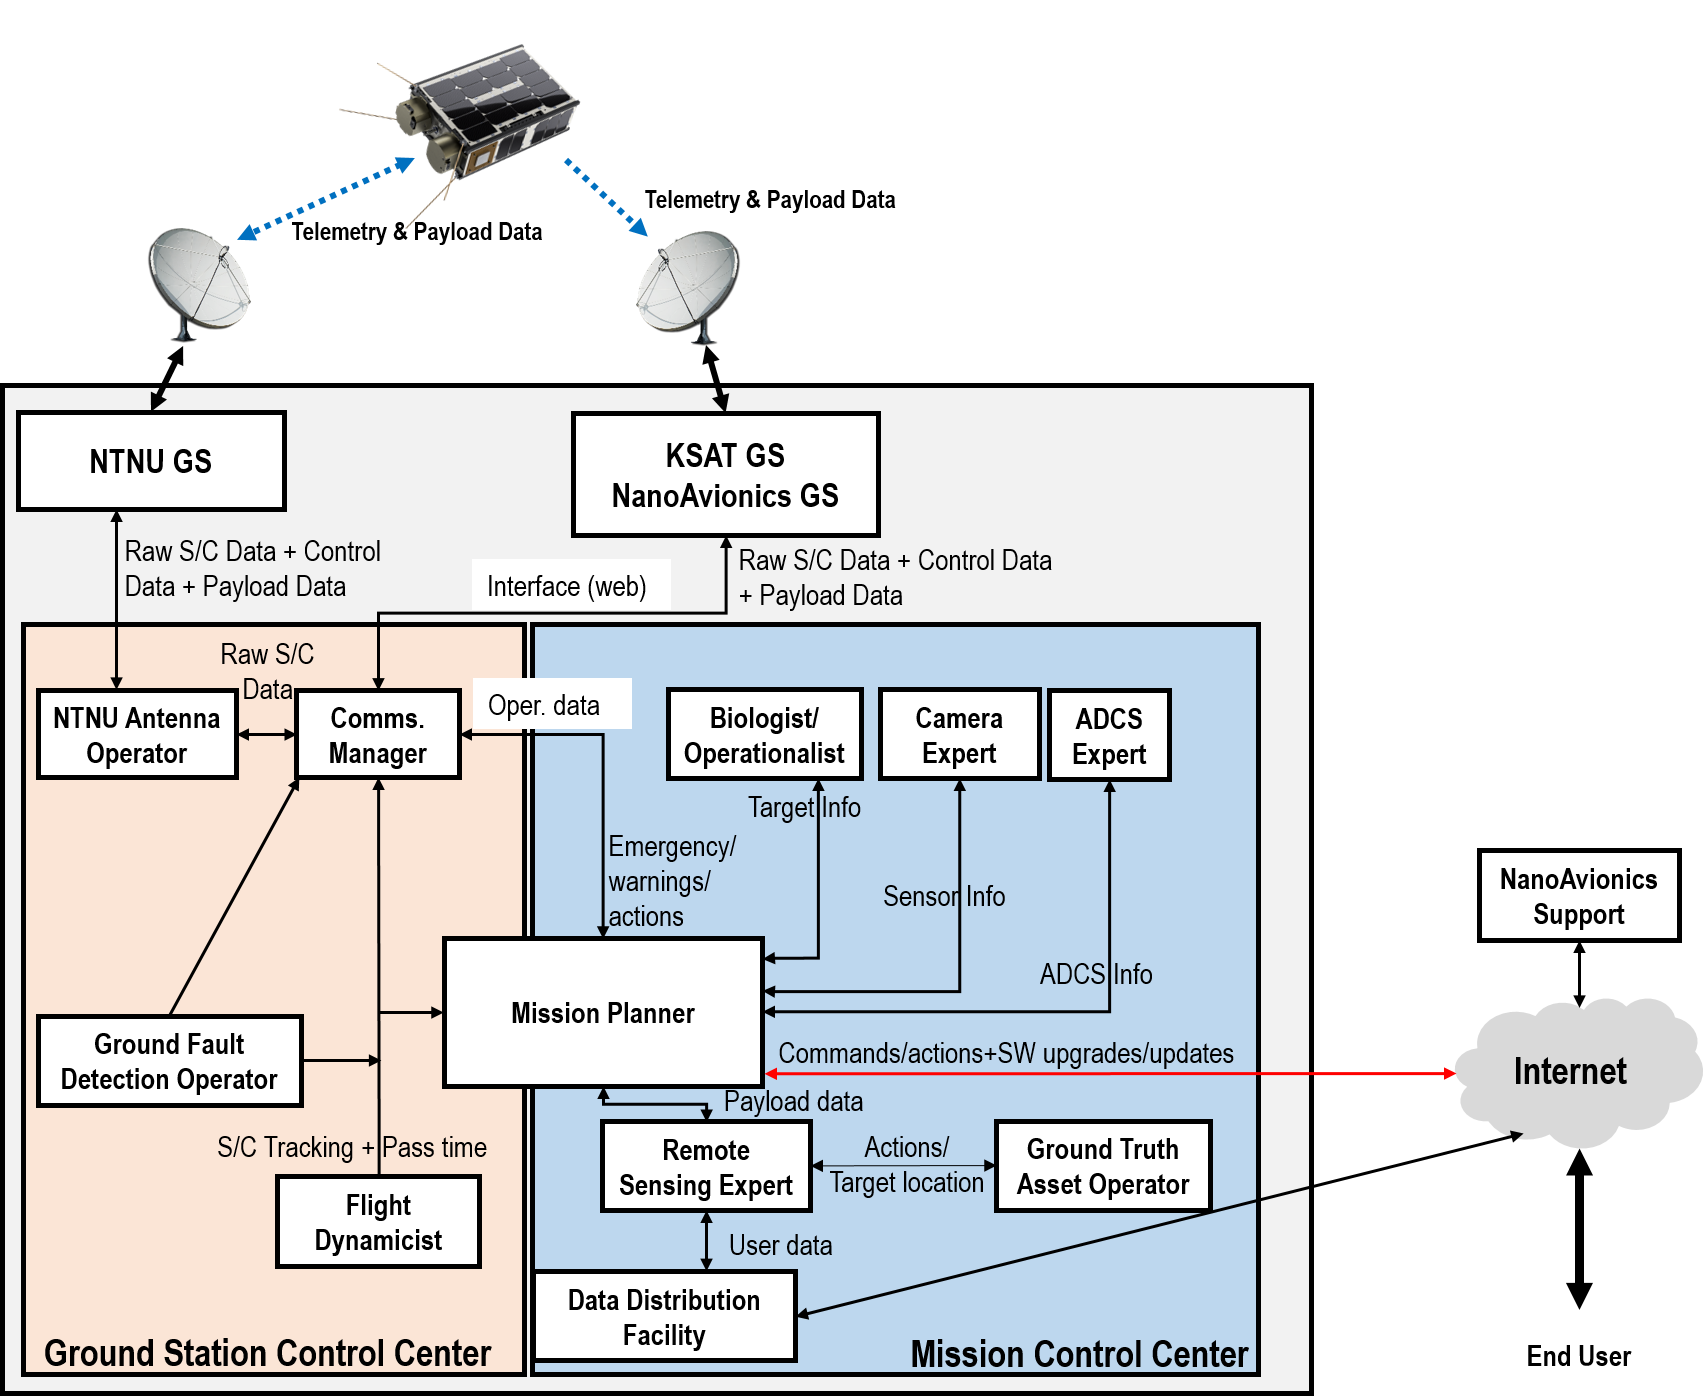
\includegraphics[width=80mm,angle=0]{figs/HYPSO_GS.png}
% %     \caption{HYPSO Ground Segment Architecture.}
% %     \label{fig:hypso-GS}
% % \end{center}
% % \end{figure}

% In order to facilitate the agility needed for mission operations, the system must make use of ground station gateways (GWS) at different locations to reduce the communication revisit time. The mission operations center (MOC) will be located at NTNU, co-located with one combined S-band and one UHF station. Other S-band stations are available through the KSAT Lite network, as well as through NanoAvionics and partners. 

% The use of the GWS is coordinated by the mission control software (MCS, NanoAvionics). This software acts as a router between the MOC, GWSs and the satellite. The MCS will route data intended for the satellite through the correct GWS during a pass. Data from the satellite is likewise routed from through the GWS and MCS to the end user. 
% \begin{figure*}
%     \centering
%     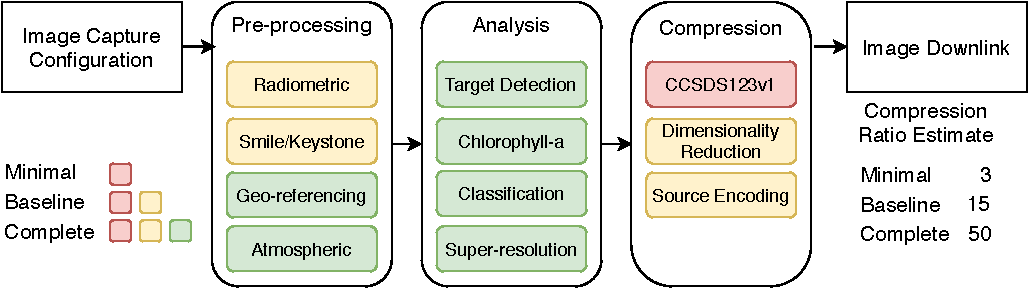
\includegraphics[width = 0.9\textwidth]{figs/img_processing/pipeline_figure_concept_paper.pdf}
%     \caption{Illustration of proposed imaging pipelines. Minimal for launch, baseline for the first updates, and complete when reached maturity.}
%     \label{fig:image-processing-pipelines}
% \end{figure*}

\begin{figure*}
    \centering
    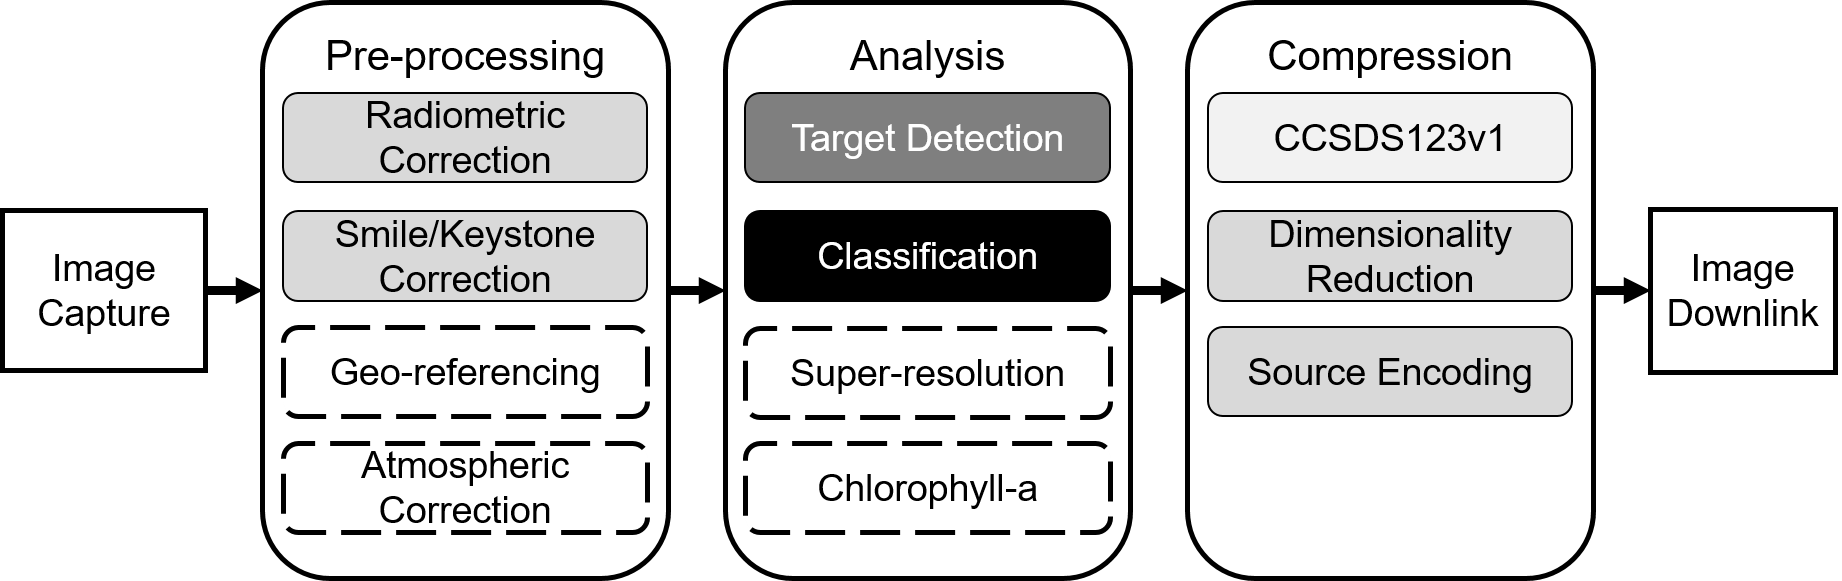
\includegraphics[width = 0.8\textwidth]{figs/img_processing/image-processing-pipeline.png}
    \caption{Diagram of the proposed imaging processing pipelines. Lightest gray block represents MOBIP, darker gray blocks represent BOBIP, darkest gray block represents TOBIP and black block represents COBIP. The dashed blocks represent modules planned for advanced image processing pipelines.}
    \label{fig:image-processing-pipelines}
\end{figure*}
\subsection{Image processing architecture}
 Figure \ref{fig:image-processing-pipelines} illustrates a diagram of the HYPSO-1's modular image processing architecture which is implemented on the OPU. 
% The modular design allows the operators to switch between the modules as needed. 
The modules can be arranged flexibly with specific orderings that each generate tailored data products, designated as image processing pipelines.
% Binning and subsampling is incorporated into the imager configuration itself to enable higher FPS with lower data traffic and so the most raw data is reduced before the image processing pipelines begin.
The estimated data size reduction factors for each pipeline are shown in Table \ref{tab:data-reduction}.
\begin{table}[htbp]
	\caption{Estimated Data Reduction of Image Processing Pipelines}
	\label{tab:data-reduction}
	\centering
	\begin{tabular}{l |r}
	\hline
	Pipeline & Factor \\
	\hline
    Minimal On-Board Image Processing (MOBIP) & 3 \\
    Baseline On-Board Image Processing (BOBIP) & 14.8 \\
    Target Detection On-Board Image Processing (TOBIP) & 49.9 \\
    Classification On-Board Image Processing (COBIP) & 93.2 \\
    \hline
\end{tabular}
\end{table}
% The planned on-board processing is divided into multiple different pipelines, illustrated in figure \ref{fig:image-processing-pipelines}, that share a basic structure, i.e. some level of processing has to be performed regardless, while others may only improve the timeliness of desired data products or reduce the expected data volume to be down-linked. In the subsequent section a high-level description of the software used and planned in the on-board processing is provided.
% \subsubsection{Settings \& Pre-processing}
% The HSI camera will collect spectrograms at a rate of 15-40 Hz. 
% The data rate is limited by the GigE that connects the camera to the breakout board, but by reducing the area of interest or doing sub-sampling in the spectral dimension, the rate at which frames are collected is adjusted \cite{varntresk2019assembly}. 
% It is expected that the imaging sensor of the HSI camera will have some distortions as a result of the optics, and that the sensitivity of given pixels will change over time. 
% Pre-processing, the initial stage of the imaging pipeline seeks to accommodate these undesirable artifacts.
\begin{table*}[htbp]
	\caption{Uncompressed Data Products*} %\textcolor{red}{Update this Re. Table VI}}
	\label{tab:data-products}
	\centering
	\begin{tabular}{l | r r r r}
	\hline
	& Bands & Pixel size ($\rm{bits}$) & Signatures ($\rm{MB}$) & Total ($\rm{MB}$) \\
	\hline
	Raw & 1074 & $16$& - & 1716 \\
	Binned & 119 & $16$ & - & 190.1 \\
	Dimensionality reduced & 20 & $16$ & - & 32.0 \\
	Classification (16 classes) & 1 & $4$ & 0.003 & 0.40 \\
	Classification (256 classes) & 1 & $8$ & 0.051 & 0.85 \\
	Target detection (only ACE) & 1 & $16$ & - & 1.60\\
	Target detection (with abundance) & 2 & $16$ & - & 3.20 \\
	Target coordinates (top 100) & n/a & $16$ & - & 0.001 \\
	\hline
	\end{tabular}
	
	\begin{tabular}{c}
		*assuming 1168$\times$684 spatial pixels. %\hl{what about spatial compression - jpeg?}
	\end{tabular}
	\vspace*{-\baselineskip}

\end{table*}
\subsubsection{Minimal on-board image processing}
The minimal on-board image processing (MOBIP) pipeline consists of the CCSDS123v1 lossless compression algorithm which is implemented on the OPU's FPGA but can also run on the CPU \cite{Fjeldtvedt2018, orlandic_parallel_2019}. The data size is reduced by a factor of approximately 3. Without loss of spatial or spectral information, the MOBIP data product can be provided to end users who wish to process the data further.  

\subsubsection{Baseline on-board image processing}
The baseline on-board image processing (BOBIP) pipeline adds two important modules to MOBIP, before source encoding and compression are applied. 
The first is a smile and keystone correction, which adjusts images to account for systematic optical and measurement errors inherent to the imager \cite{Henriksen2019}. 

Second is dimensionality reduction, which allows for control of data size while retaining most of the information of the image by adjusting the number of selected reducted bands. \cite{Vit17}. 
% \hl{removing noise-like and redundant components }. 
The smile and keystone correction is applied before the dimensionality reduction to prevent the latter from intertwining systematic, but reversible artifacts irrevocably with the data. For image processing modules beyond BOBIP, dimensionality reduction will increase the computational speed because there will be fewer bands to process \cite{Bakken2019SPIE}.

% \textcolor{red}{For BOBIP, the On-the-Fly-Processing (OTFP) algorithm cam be used as dimensionality reduction because it allows for accurate reconstruction of the hypserspectral information with a minimal number of bands \cite{Vit17}. 
% The residuals from the dimensionality reduction can also be downlinked occasionally and analysed to provide insight about the components removed from the data.
% Once it is rigorously tested and approved, the BOBIP pipeline will provide the nominal data products. 
% For BOBIP the number of selected bands is expected to be about 20.

\subsubsection{Target detection on-board image processing}
Another way to expand MOBIP or BOBIP is to add a target detection (TD) module before compression, named target detection on-board processing (TOBIP) pipeline. Hyperspectral data is amenable to target detection because of its numerous channels \cite{Manolakis2002, Manolakis2005}. One target signature will result in a probability map, or a heat map, of its occurrence across the scene. Multiple target signatures can be represented as separate bands. 
% By incorporating spectral information about the background scene, TD algorithms can locate sub-pixel spectral signatures.
% The 2D heat maps produced by TD are small in data size and can be immediately used to guide in-situ agents without requiring additional processing on ground. 
The Adaptive Cosine Estimator (ACE) is a target detection algorithm for hyperspectral images that is often used to determine the likelihood of a pixel containing a particular spectral signature. 
Both software and software-hardware co-design versions of the algorithm have been developed for OPU. Computing acceleration provided by the OPU's FPGA results in a speedup factor of about $28$ times relative to software implementations \cite{dijehw19_meco}. Effective use of ACE requires a-priori knowledge about the target spectra to be observed. 
% \textcolor{orange}{A spectrum can either be estimated from data in the lab, which is susceptible to calibration inconsistencies between the lab camera and the satellite camera, or it can be estimated directly from the satellite data, so that the target spectrum and input data traverse similar optical paths \hl{?}}. 
A complementary algorithm, the abundance estimator, can be used to estimate how much of a pixel is contained by a target signature. 
For some applications, such as chlorophyll estimation, the abundance estimator itself will be the most relevant component of the data. 

The maxima in a heat map show the pixel locations where it is most probable that a particular target signature is present. Instead of downlinking the entire heat map it is possible transfer only the pixel coordinates of a number of the maxima. If the coordinates are geo-referenced, the in-situ agents can quickly travel to the location of these maxima to inspect in more detail. For example, if the location of the 100 largest local maxima of the map are downlinked together with their latitudes and longitudes, the total data package will only be about $1 \hspace{3pt} \rm{kB}$, shown in Table \ref{tab:data-products}. % The small size of this data product can be quickly downlinked after image acquisition, and for that reason it will enhance the capability of in-situ agents to track dynamic ocean phenomena.
\subsubsection{Classification on-board image processing}
Alternative to TOBIP is the classification on-board image processing (COBIP) pipeline with a classification algorithm that separates the pixels of a hyperspectral image into different classes \cite{Alcolea_2020}. With fewer than 16 classes, it is possible to represent each pixel with a 4 bit integer whereas up to 256 classes can be represented with 8 bits. Representative spectra for each class will also be downlinked. 

Graph-based clustering, an unsupervised method, will be adapted to be run on the OPU as the initial classification algorithm because of its flexibility and it does not require training data \cite{Wang2017}.
Once a database of hyperspectral images is acquired and labelled, a supervised classification algorithm will be incorporated as an alternative.
Recent experiments have shown that gradient boosting decision trees achieve a good balance of accuracy and computational requirements for on-board processing \cite{Alcolea_2020}.
\subsection{Advanced on-board image processing pipelines}
Additional planned algorithms, some of them depicted in dashed blocks in Figure \ref{fig:image-processing-pipelines}, are still in development and may be uploaded on the OPU while HYPSO-1 is in orbit and implemented in a similar successive mission. 
The planned algorithms include image registration, motion-blur correction, geo-referencing, atmospheric correction, and super-resolution, some of them slated to be run on ground. 
% Several of these kinds of algorithms utilize the RGB camera in addition to the hyperspectral imager, so it must be drawn into the image processing pipelines. 
Depending on the end user and target area, different tailored data products will be desired and more modules can be added to the image processing architecture based on these needs. We discuss a few selected algorithms next.

\subsubsection{Image registration and geo-referencing}
In general, even very simple algorithms for registration and geo-referencing require more computational power than is available on-board the HYPSO-1 \cite{Opsahl_2011}. Here, we refer to image registration as the determination of the relative separation of the individual pixels, or sometimes named orthorectification, and geo-referencing as the process of assigning all the pixels to latitude and longitude coordinates. For example, registration is necessary to enable any spatial-spectral methods in image classification, which tend to be more accurate than those that rely only on spectral information. Similarly, to downlink the target detection local maxima coordinates, it is necessary to determine what the latitude and longitude of the relevant pixels. For on-board operation, a simple ray-tracing method will be adapted, which has been prototyped on the ground for joint registration and geo-referencing, similar to the one described in \cite{Schlapfer2002} but with a flat elevation model for the water surface. 
% However, it is expected that more advanced perturbative techniques may be required, and those techniques will initially be run on the ground. 

\subsubsection{Super-resolution}
Super-resolution algorithms are being adapted to enhance the spatial resolution in the images as described in \cite{Park2003}, and may provide high-accuracy and resolution. The initial prototypes for super-resolution model require a measurement process, e.g. determining the point-spread function, and then use that to infer the image at higher spatial resolution \cite{Garrett2019}. The prototypes are based on methods that come from multi-frame super-resolution because of its similarity with the irregularly-sampled data from the slew maneuver \cite{stark_high-resolution_1989, farsiu_fast_2004}. 
Although these super-resolution algorithms do improve the resolution somewhat, they are susceptible to noise, digitization, compression and inaccuracies in the estimate of the point spread function \cite{Baker2002,Kohler2019}. 
However, some of these measurement-based super-resolution methods have previously been successfully applied to remote sensing data \cite{clarisse2019tracking}. 

Prior-based super-resolution techniques overcome the limitations of measurement-based reconstruction techniques by supplementing the input pixels with additional expectations about image statistics. 
Examples of general prior-based techniques include sparse image representations \cite{Yang2010}, and convolutional neural nets \cite{Kim_2016_CVPR,Anwar2020}. 
Some of these produce plausible images at magnification factors of up to 8 times, and even a factor of 6 times. However, these techniques are specifically designed for hyperspectral data. 

On the other hand, dimensionality reduction-based super-resolution techniques unique to hyperspectral imagery have been developed as well \cite{Akgun2005}. Recently, numerous multispectral-hyperspectral fusion techniques have been proposed to enhance the resolution of the latter \cite{Lanaras_2015_ICCV, Yokoya2017}. For utilizing super-resolution in the HYPSO-1 mission, it is necessary to determine how it can be incorporated into a framework with classification or target detection.

\subsubsection{Upload/reprogram Capability}
Both the software and FPGA configurations are planned to be updated during the operation of the satellite \cite{Gjersund2020}. 
The software update must be stringently tested on the ground, both in terms of timeliness and computing resources, before uploading it which can take several passes to complete. 
The OPU retains \textit{golden image}, a version of the operating system and software known to have worked, that it will revert to in case of an update failure. 

\subsubsection{Ground Processing Pipeline}
Similar and extended image processing pipelines should operate on the ground to (a) adjust, fine-tune and prepare data for end users; (b) assist in in-orbit calibration of the hyperspectral imager; and (c) to test algorithms rigorously before uploading them to the satellite for on-board image processing. 
Some of the components of the pipeline such as geo-referencing, atmospheric correction and super-resolution are also amenable to being applied to the data on ground because they require access to reference libraries and are more computationally expensive than the other modules presented.
% \begin{table}[htbp]
% 	\caption{Data budget}
% 	\label{tab:data-budget}
% 	\centering
% 			\begin{tabular}{l r r r r}
% 				\hline
% 				S-band TX Data Rate & $1 \hspace{3pt} \rm{Mbps}$ & & & \\ 
% 				S-band RX Data Rate & $0.04 \hspace{3pt} \rm{Mbps}$ & & & \\ 
% 			   CAN Buffer Speed & $0.4 \hspace{3pt} \rm{Mbps}$ & & & \\
% 			   \hline
% 			    & Upload & TM & Data A & Data B \\
% 			  \hline
% 		    Data Size (MB) & 0.1 & 0.1 & 100.29 & 11.06 \\
% 			CAN Transfer Time (min) & 0.03  & 0.03 & 33.43 & 3.69 \\
% 			Downlink Time (min) & - & 0.01 & 13.37 & 1.47 \\
% 		    Uplink Time (min) & 0.33 & - & - & -  \\
% 		    Orbits Required & 0.0039 & 0.0021 & 2.58 & 0.08 \\
% 				\hline
% 				\end{tabular}
% \end{table}

% \begin{table}[htbp]
% 	\caption{Data Constraints}
% 	\label{tab:data-constraints}
% 	\centering
% 	\begin{tabular}{l r }
%         \hline
%         Available onboard processing time	& $347.26 \hspace{3pt} \rm{s}$\\			
%         Available onboard transfer time &	$2005.80 \hspace{3pt} \rm{s}$\\			
%         Available downlink time &	$1320 \hspace{3pt} \rm{s}$ \\				
%         Maximum data transferred per orbit &	$100.29 \hspace{3pt} \rm{MB}$ \\
%         Total downlink per orbit (incl. headers) &	$165 \hspace{3pt} \rm{MB}$ \\				
%         SD card storage space available	& $24 \hspace{3pt} \rm{GB}$ \\
%         \hline
%     \end{tabular}
% \end{table}
\begin{table*}[htbp]
	\caption{Summary of selected hyperspectral imager mode performance}
	\label{tab:data-types}
	\centering
	\begin{tabular}{l r r r r r}
        Type &	Mode A & Mode B & Mode C & Mode D & Mode E \\ % OK
        \hline
        ADCS Mode &	Slew ($\theta_0=20^{\circ}$) & Slew ($\theta_0=20^{\circ}$) & Slew ($\theta_0=20^{\circ}$) & Nadir & Nadir \\ % OK
        AoI (pixels) &	$1074\times684$ & $1074\times684$ & $1074\times1194$ & $1074\times1194$ & $1936\times1216$\\ % OK
        Binning, $B_\lambda$ (pixels) &	9 & 18 & 9 & 9 & 1 \\ % OK
        % Sub-sampling (pixels) &	1 &	1 &	1 &	1 & 1\\ % OK
        Spectral range ($\rm{nm}$) & $400-800$ & $400-800$ & $400-800$ & $400-800$ & $276-1006$ \\ % OK 
        Spectral bands & 119 & 59 & 119 & 119 & 220 \\ % OK 
        Bandpass ($\rm{nm}$) & 3.33 & 6.67 & 3.33 & 3.33 & 3.33 \\ % OK
        FPS & 22 & 15 & 12 & 12 & 3 \\ % OK
        Exposure time, $\tau$ ($\rm{ms}$) &	41.45 & 49.10 & 49.10 & 49.10 &	49.10 \\ % OK
        Scan duration ($\rm{s}$) & 53.08 & 53.08 & 57.00 & 9.19 & 1.0 \\ % OK
        Number of frames & 1168 & 797 & 685 & 111 & 3 \\
        SNR of target @$471 \hspace{3pt} \rm{nm}$, nadir & 107.87 & 166.52 & 117.75 & 117.75 & 40.00 \\
        Scan distance, along-track ($\rm{km}$) & 40.08 & 40.08 & 69.97 & 69.97 & 7.60  \\ % OK
        Spatial resolution, along-track, nadir ($\rm{m}$) & 542.9 & 550.9 & 573.1 & 873.8 & 873.8  \\
        Swath width, nadir ($\rm{km}$) & 40.08 & 40.08 & 69.97 & 69.97 & 69.97 \\ % OK
        Spatial resolution, cross-track, nadir ($\rm{m}$) & 58.60	& 58.60 & 58.60 & 58.60 & 58.60 \\
        SGSD, along-track ($\rm{m}$) & 47.09 & 69.07 & 124.08 & 634.39 & 2537.56 \\
        Data size, Raw ($\rm{MB}$) & 190.67 & 65.05 & 195.20 & 31.63 & 14.13 \\
        \hline
        Data size, MOBIP ($\rm{MB}$) & 63.56 & 21.68 & 65.07 & 10.54 & 4.71 \\
        Onboard processing time ($\rm{s}$) & 1.64 & 1.22	& 1.65 & 1.11 & 1.05 \\
        CAN transfer time ($\rm{min}$) & 21.19 & 7.23 & 21.69	& 3.51 & 1.57 \\
        Downlink time ($\rm{min}$) & 8.47 & 2.89 &	8.68 &	1.41 & 0.63 \\
        \hline
        Data size, BOBIP ($\rm{MB}$) & 12.82 & 8.82 & 13.12 & 2.13 & 0.51 \\
        Onboard processing time ($\rm{s}$) & 49.30 & 17.48	& 50.45 & 9.01 & 4.58 \\
        CAN transfer time ($\rm{min}$) & 4.27 & 2.94 & 4.37 & 0.71 & 0.17 \\
        Downlink time ($\rm{min}$) & 1.71 & 1.18 & 1.75 & 0.28 & 0.07 \\
        \hline
        Data size, TOBIP ($\rm{MB}$) & 3.82 & 1.30 & 3.91 &	0.63 & 0.28 \\
        Onboard processing time ($\rm{s}$) & 96.97 & 33.74	& 99.25 & 16.92 & 8.11 \\
        CAN transfer time ($\rm{min}$) & 1.27 & 0.43 & 1.30 & 0.21 & 0.09 \\
        Downlink time ($\rm{min}$) & 0.51 & 0.17 & 0.52 & 0.08 & 0.04 \\
        \hline
        Data size, COBIP ($\rm{MB}$) & 2.05 & 0.70 & 2.09 &	0.34 & 0.15 \\
        Onboard processing time ($\rm{s}$) & 96.97 & 33.74	& 99.25 & 16.92 & 8.11 \\
        CAN transfer time ($\rm{min}$) & 0.68 & 0.23 & 0.70 & 0.11 & 0.05 \\
        Downlink time ($\rm{min}$) & 0.27 & 0.09 & 0.28 & 0.05 & 0.02 \\
        \hline
	\end{tabular}
\end{table*}
% \begin{table*}[htbp]
% 	\caption{Data Types}
% 	\label{tab:data-types}
% 	\centering
% 	\begin{tabular}{l r r r r r}
%         \hline
%         Allowed onboard processing time	& $347.26 \hspace{3pt} \rm{s}$ & & & &\\			
%         Allowed onboard transfer time &	$2005.80 \hspace{3pt} \rm{s}$ & & & &\\			
%         Allowed downlink time &	$1320 \hspace{3pt} \rm{s}$ & & & &\\				
%         Allowed data size to transfer per orbit &	$100.29 \hspace{3pt} \rm{MB}$ & & & &\\
%         Allowed to downlink per orbit &	$165 \hspace{3pt} \rm{MB}$ & & & &\\				
%         Allowed to store (SD card)	& $24 \hspace{3pt} \rm{GB}$ & & & &\\					
%         \hline
%         Type &	Data A &	Data B &	Data C &	Data D &	Data E \\
%         \hline
%         ADCS Mode &	Slew &	Slew &	Nadir &	Slew &	Slew \\
%         AoI (pixels) &	$1200\times720$ &	$1200\times720$ &	$1200\times720$ &	? &	?\\
%         FPS &	20 &	20 &	30 &	20 &	20\\
%         Maximum exposure, $\tau$ ($\rm{ms}$) &	50 &	50 &	33 &	50 &	50\\
%         Binning, $B_\lambda$ (pixels) &	3 &	3 &	3 &	? &	12 \\
%         Sub-sampling (pixels) &	4 &	4 &	4 &	? &	1 \\
%         Spectral Bands &	161 &	20 &	161 &	161 &	161 \\
%         Number of frames &	1139 &	1139 &	276 &	1139 &	1139 \\
%         \hline
%         Level 1 data size ($\rm{MB}$) (1/2) &	87.21 &	19.234 &	25.07 &	? &	? \\
%         Time required to transfer ($\rm{min}$)	& 29.07 &	6.4113 &	8.3567 & & \\		
%         Time required to download ($\rm{min}$)	& 11.628 &	2.5645 &	3.34 & & \\		
%         Number of datacubes per orbit &	1.89 & & & & \\				
%         \hline
%         Level 2 data size ($\rm{MB}$) (1/2) &	43.605 & 	9.617 &	12.535 & & \\		
%         Time required to transfer ($\rm{min}$)	& 14.535 &	3.2057 &	4.1783 & & \\		
%         Time required to download ($\rm{min}$)	& 5.814	& 1.2823 &	1.6713 & & \\		
%         Number of datacubes per orbit & & & & & \\					
%         \hline
%         Level 3 data size ($\rm{MB}$) (1/10) &	4.3605 & 0.962 &	1.2535 & & \\		
%         Time required to transfer ($\rm{min}$) &	1.4535 &	0.3207 &	0.4178 & & \\		
%         Time required to download ($\rm{min}$) &	0.5814 &	0.171 &	0.1671 & & \\		
%         Number of datacubes per orbit &	17 & & & & \\ 
%         \hline
% 	\end{tabular}
% \end{table*}

% \begin{table*}[htbp]
% 	\caption{Latency for Mode A Data}
% 	\label{tab:scenario-2b}
% 	\centering
% 	\begin{tabular}{l l l r}
%         \hline
%         Sequence & Start time & End time & Duration ($\rm{s}$) \\	
%         \hline
%         Orbit 1 & & & \\
%         \hline
%     	HSI scan & 10:11:17.00 & 10:12:10.36 & 53.36 \\
%     	Onboard Processing & 10:12:10.36 & 10:12:12.04 &  1.68 \\
%     	CAN Transfer & 10:12:12.04 & 10:34:58.06 & 1366.02 \\
%         Cruise & 10:34:58.06 & 10:52:18.36 & 1040.30 \\
%         Eclipse & 10:52:18.36 & 11:27:10.34 & 2091.98 \\
%         \hline
%         Orbit 2 & & & \\
%         \hline
%         Exit Eclipse & 11:27:10.30 &	11:39:51.17 & 760.87 \\
%         Downlink to KSAT Svalbard & 11:39:51.17 & 11:43:52.46 & 241.29 \\
%         Downlink to NTNU & 11:43:52.46	& 11:48:57.57 & 305.11 \\
%         \hline
%         Total latency ($\rm{hrs}$) & & & 1.63 \\
%         \hline
%     \end{tabular}
% \end{table*}
\begin{table*}[htbp]
	\caption{Latency for Mode A data}
	\label{tab:scenario-2b}
	\centering
	\begin{tabular}{l | l r |l  r|l r|l r}
	    \hline
         & MOBIP & ($63.56 \hspace{3pt} \rm{MB}$) & BOBIP  & ($12.82 \hspace{3pt} \rm{MB}$) & TOBIP & ($3.82 \hspace{3pt} \rm{MB}$) & COBIP & ($2.05 \hspace{3pt} \rm{MB}$) \\		
        \hline
        Sequence & Start time & Duration ($\rm{s}$) & Start time & Duration ($\rm{s}$) & Start time & Duration ($\rm{s}$) & Start time & Duration ($\rm{s}$) \\	
        \hline
        Orbit 1 & & & & & & & & \\
        \hline
    	HSI scan & 10:14:15.00 & 53.08 & 10:14:15.00 & 53.08 & 10:14:15.00 & 53.08 & 10:14:15.00 & 53.08 \\
    	Onboard Processing & 10:15:08.08 &  1.64 & 10:15:08.08 & 49.30 & 10:15:08.08 & 96.97 & 10:15:08.08 & 96.97  \\
    	CAN Transfer & 10:15:09.14 & 1271.16 & 10:15:57.38 & 256.37 & 10:16:45.05 & 76.32 & 10:16:45.05 & 40.93 \\
        Downlink to NTNU & - & - & - & - & 10:18:01.37 & 30.53 & 10:17:25.98 & 16.37 \\
        Downlink to KSAT Spain & - & - & 10:20:13.75 & 102.55 & - & - & - & - \\
        Cruise & 10:36:20.30 & 1316.47 & - & - &- & - & - & - \\
        Eclipse & 10:58:16.77 & 2051.50 & - & - &-  & - & - & - \\
        \hline
        Orbit 2 & & & & & & & & \\
        \hline
        Exit Eclipse & 11:32:28.27 & 601.35 & - & - & - & - & - & - \\
        Downlink to KSAT Svalbard & 11:42:29.61 & 242.65 & - & - & - & - & - & - \\
        Downlink to NTNU & 11:46:32.26	& 265.82 & - & - & - & - & - & - \\
        \hline
        Total latency ($\rm{min}$) & & 96.73 & & 7.69 & & 4.28 & & 3.46 \\
        \hline
    \end{tabular}
\end{table*}
% \begin{table*}[htbp]
% 	\caption{Latency for Mode A Data - w/o CAN overhead}
% 	\label{tab:scenario-2b}
% 	\centering
% 	\begin{tabular}{l l l r}
%         \hline
%         Sequence & Start time & End time & Duration ($\rm{s}$) \\	
%         \hline
%     	HSI scan & 10:11:17.00 & 10:12:10.36 & 53.36 \\
%     	Onboard Processing & 10:12:10.36 & 10:12:12.04 &  1.68  \\
%         Downlink to NTNU &	10:12:12.04 & 10:17:06.50 &	294.46 \\
%         Downlink to KSAT Spain & 10:17:06.50 & 10:21:18.44 &	251.94 \\
%         \hline
%         Total latency ($\rm{min}$) & & & 10.03 \\
%         \hline
%     \end{tabular}
% \end{table*}
\begin{table*}[htbp]
	\caption{Latency for Mode A data - w/o CAN overhead}
	\label{tab:scenario-2c}
	\centering
	\begin{tabular}{l | l r |l  r|l r |l r}
	    \hline
         & MOBIP & ($63.56 \hspace{3pt} \rm{MB}$) & BOBIP  & ($12.82 \hspace{3pt} \rm{MB}$) & TOBIP & ($3.82 \hspace{3pt} \rm{MB}$) & COBIP & ($2.05 \hspace{3pt} \rm{MB}$) \\	
        \hline
        Sequence & Start time & Duration ($\rm{s}$) & Start time & Duration ($\rm{s}$) & Start time & Duration ($\rm{s}$) & Start time & Duration ($\rm{s}$) \\	
        \hline
    	HSI scan & 10:14:15.00 & 53.08 & 10:14:15.00 & 53.08 & 10:14:15.00 & 53.08 & 10:14:15.00 & 53.08 \\
    	Onboard Processing & 10:15:08.08 &  1.64 & 10:15:08.08 & 49.30 & 10:15:08.08 & 96.97 & 10:15:08.08 & 96.97  \\
        Downlink to NTNU & 10:15:09.14 &	243.42 & 10:15:57.38 & 102.55 & 10:16:45.05 &	30.53 & 10:16:45.05 & 16.37 \\
        Downlink to KSAT Spain & 10:19:12.56 &	265.05 & - &	- & - &	- & - & - \\
        \hline
        Total latency ($\rm{min}$) & & 9.39 & & 3.42 & & 3.01 & & 2.77 \\
        \hline
    \end{tabular}
\end{table*}
% \subsubsection{Ground Station Network}

% \subsubsection{Mission Control Center (TENTATIVE)}
% \hl{Roger, Mariusz,  \\}
% \subsubsection{Ground Image Processing}
% \hl{Joe, Sivert \\}
% \subsubsection{Data Dissemination (TENTATIVE)}
% \hl{Joe, Mariusz, Sivert \\}

% \subsubsection{Image Processing - Preliminary Results}
% \hl{Sivert, Joe \\}
% Super-resolution algorithms may be developed to enhance the spatial resolution \cite{Park2003, Garrett2019} and provide improved detectability of features of interest. 
% \subsubsection{Results with Robotic In-situ Agents (TENTATIVE)}
% \hl{Sivert, Joe \\}
\subsection{Data Latency}
% Reaching negative remaining power assumes that HYPSO-1 operates beyond what is required which may be detrimental for the battery charging capacity due to high depth-of-discharge over repeated orbits and shall be avoided, e.g. processing over longer time or downlinking more data than the time allocated.

% Given the condition where all of the following sequences shall be executed in the CONOPS
% \begin{itemize}
%     \item uplinking necessary updates, e.g. scripts with TC and camera settings;
%     \item scanning a $70 \hspace{3pt} \rm{km} \times 70 \hspace{3pt} \rm{km}$ target area while slewing at $\omega_y=0.7025 \hspace{3pt} \rm{deg/s}$ from $\theta=20 \hspace{3pt} \rm{deg}$ to $\theta=-20 \hspace{3pt} \rm{deg}$;
%     \item Buffering acquired payload data to radio if necessary with CAN data rate of $0.4 \hspace{3pt} \rm{Mbps}$ including overhead and margin; and
%     \item Downlinking on-board compressed data immediately to next available ground station with S-band data rate of $1 \hspace{3pt} \rm{Mbps}$ including overhead, $15 \%$ margin data size and assuming $10 \hspace{3pt} \rm{deg}$ ground station antenna elevation.
% \end{itemize}
% \noindent and considering the constraints with power budget, data rates through radio and CAN as well as available ground station passes, then each orbit allows for the HSI to capture up to 1140 frames during a total image acquisition time for 57 seconds and consecutively downlinking the data to the nearby ground stations after acquisition. To enable this, the camera parameters may be set to
% \begin{itemize}
%     \item 25 FPS
%     \item AoI of $1280 \times 720$ pixels
%     \item Binning of $B_\lambda=6$ and $B_y=1$
%     \item Sub-sampling of 2 adjacent pixels in the spectral direction
% \end{itemize}
% which results in a data size of $0.144 \hspace{3pt} \rm{MB}$ per frame. Further compressed data results in the size of $0.072 \hspace{3pt} \rm{MB}$ per frame, latter representing the total size for Data A and Data B in Table \ref{tab:data-budget}. For best case and considering scheduled light-duty operations during eclipse, Data A download may be completed in the next orbit pass, i.e. after approximately $1 \hspace{3pt} \rm{hr}$ and $34 \hspace{3pt} \rm{min}$. Data B may be downloaded in the first pass in $1 \hspace{3pt} \rm{min}$ and $28 \hspace{3pt} \rm{s}$. 
% Because of the large size of hyperspectral data products, the data budget limits the number of frames that can be captured, transferred on-board, and downlinked, and, further, limits the timeliness with which they can be downlinked.
% For example, without any AoI cropping or post-processing (binning, compression), the raw data of 500 frames from one slew maneuver will be about $2.36 \hspace{3pt} \rm{GB}$ which is $4.71 \hspace{3pt} \rm{MB}$ per frame. Using the S-band downlink data rate, this would require more than $5 \hspace{3pt} \rm{hrs}$ of continuous transmission to downlink which is beyond the power budget capability and latency requirements.

% Short time between acquisition and data distribution to end users, specifically in less than $3 \hspace{3pt} \rm{hrs}$, is a critical success criteria for demonstration of the HYPSO-1 mission. 
Table \ref{tab:data-types} shows the selected hyperspectral imager modes and the corresponding performance and data size reduction for MOBIP, BOBIP, TOBIP and COBIP. The choice of AoI and binning operations decides the allowed FPS setting for each mode. Mode A and B provide higher spatial resolution but narrower FoV for a target area size of approximately $40 \hspace{3pt} \rm{km}$ by $40 \hspace{3pt} \rm{km}$, while Mode C and D provide coarser spatial resolution and wider FoV for a target area size of approximately $70 \hspace{3pt} \rm{km}$ by $70 \hspace{3pt} \rm{km}$. Mode A, B, C and D have $1074$ out of $1936$ pixels in the spectral direction and cover the spectral range of $400-800 \hspace{3pt} \rm{nm}$. Mode E, with full AoI, is used in the commissioning phase and for in-orbit sensor characterization and calibration to be performed regularly. "On-board processing time", "CAN transfer time" and "Downlink time" represent the collective time it for the image processing pipelines, completing the transfer of data between OPU to PC at speed of $0.4 \hspace{3pt} \rm{Mbps}$ and completing the downlink of data to ground through S-band radio at speed of $1 \hspace{3pt} \rm{Mbps}$, respectively. For MOBIP it takes up to $1 \hspace{3pt} \rm{s}$ to compress the data and storage of data takes up to $10 \hspace{3pt} \rm{ms/MB}$. An upper limit of allowed processing time is set at $100 \hspace{3pt} \rm{ms/MB}$ for BOBIP, TOBIP and COBIP. 

The hyperspectral imager is chosen to nominally operate with Mode A because its data product is a good compromise between spatial resolution, spectral resolution, SNR and data size. Table \ref{tab:scenario-2b} indicates the duration from acquiring 1334 hyperspectral images of a target area nearby Lofoten, Norway, to complete the download of a MOBIP, BOBIP, TOBIP and COBIP data products by the satellite operator. Results are obtained from simulations \emph{AGI Systems ToolKit (STK)} for the aforementioned orbit parameters where the date is taken to be 15 August 2021 and elevation angles for ground station antennas are $10 \hspace{3pt} \rm{deg}$. It is assumed that image acquisition, onboard processing, data transfer between OPU and PC through CAN, and data downlink through S-band radio are scheduled to be consecutive. None of the durations of each operational phase violate the power budget in Table \ref{tab:power-budget}. Keeping in mind the $3 \hspace{3pt} \rm{hrs}$ latency limit goal, for MOBIP data product with CAN overhead it would take about $1 \hspace{3pt} \rm{hr}$ and $37 \hspace{3pt} \rm{min}$ to completely download data which leaves about $1 \hspace{3pt} \rm{hr}$ and $23 \hspace{3pt} \rm{min}$ slack to further process on ground before finally presenting important and actionable information to the end users. For BOBIP, TOBIP and COBIP the latency is expected to be only a few minutes. In theory, without the CAN overhead as shown in Table \ref{tab:scenario-2c}, the latency for MOBIP would on the other hand be $9 \hspace{3pt} \rm{min}$ and $24 \hspace{3pt} \rm{s}$ and can be downlinked almost immediately after image acquisition.
